Vélbúnaður prjónavélarinn er í grófum dráttum:  nálarbeðið, sleðinn/lásinn, litaskiptirinn og mótorinn.

\begin{figure}
    \centering
    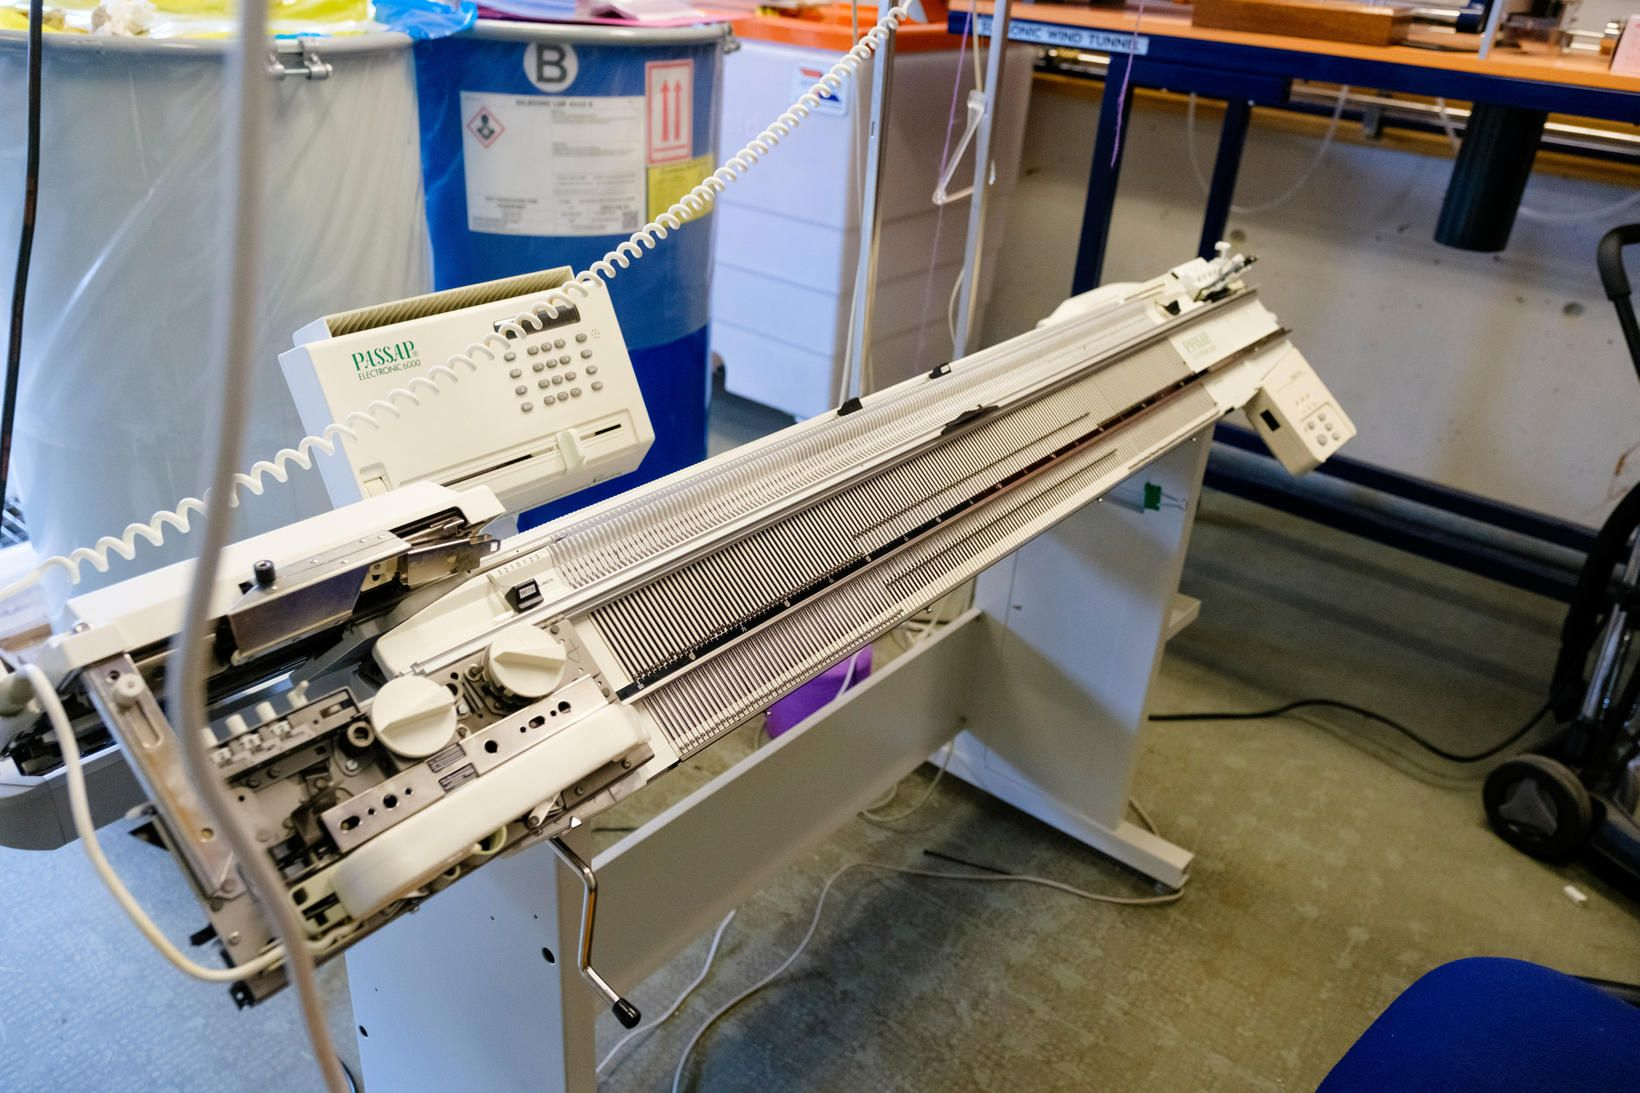
\includegraphics[width=.7\linewidth]{myndir/elli/e6000.jpg}
    \caption{\textit{Passap E6000} prjónavél - \textit{mbl.is/Kristinn Magnússon}}
    \label{fig:e6000}
\end{figure}
\subsubsection{Nálarbeð}
\begin{itemize}
    \item Braut sem sleðinn rennur eftir
    \item Nálastillara (e. pushers) sem eru undir nálunum í nálabeðinu og ýta nálunum í prjónastöðu. 
    Þeir eru notaðir til að slökkva og kveikja á nálum fyrir hverja umferð, þ.e.a.s. setja nálar í óvirka eða virka stöðu.
    \item Nálarnar sem prjóna lykkjurnar ef þær eru í réttri stöðu þegar sleðinn fer yfir þær.
    \item Nálarnar á nálabeðinu eru merktar með númeri út frá miðju. 90 nálar til vinstri og 89 nálar til hægri frá miðjunni. 179 nálar í heildina.
\end{itemize}
\subsubsection{Sleði/lás}    
    \begin{itemize}
        \item Tvo ljósaskynjara sem eru notaðir til að staðsetja sleðann á nálabeðinu.
        \item Tvo segla sem setja stöðu nálastillaranna fyrir næstu umferð.
        \item Braut sem fer með nálar í eftir tveimur mögulegum leiðum: 
        i) upp og prjónar lykkju í garninu eða ii) niður og prjónar ekki lykkju.
    \end{itemize}
\subsubsection{Litaskiptir}    
    \begin{itemize}
        \item Geymir garn.
        \item Er með einskonar takka sem sleðinn virkjar þegar hann fer yfir og skilar garni. Þá er nýtt garn sett í virka stöðu og það tekið upp á bakaleiðinni.
    \end{itemize}
\subsubsection{Mótor}    
    \begin{itemize}
        \item Snýr belti sem hefur festingu fyrir sleðann.
        \item Festingin er með segul.
        \item Það eru þrír skynjarar á umgjörðinni sem inniheldur beltið sem skynja segulinn.
    \end{itemize}
\subsection{Stýringar}
Hægt er að skipta vélbúnaðinum upp í tvö stýrikerfi. Annars vegar stýringin á mótornum sem færir sleða lásinn frá vinstri til hægri yfir nálabeðið. Hinsvegar stýringin á seglunum sem færa nálastillara á nálabeðinu upp og niður. Fyrir hvern nálastillir sem er stillt upp er lykkja prjónuð með garni fyrir þá nál í næstu umferð.
\subsubsection{Stýring nálarbeðs}
Upprunalega \textit{Passap E6000} vélin er með stjórnborð (svokölluð \textit{Form} tölva) sem er tengd með DIN-6 snúru við sleðann sem er læstur á nálabeðinu. Sleðinn er
með rafrás sem hefur ljósskynjara sem skynja göt á brautinni sem sleðinn rennur eftir. Götin eru \textit{2mm} breið og það eru \textit{3mm} á milli gata. Hver nál er \textit{5mm}. Mynd \ref{fig:original-pusher-control} er kerfismynd af kerfinu sem stýrir nálastillurunum á nálabeðinu. Upprunalega stjórnborðinu var skipt út fyrir \textit{Arduino} með \textit{12v} spennubreyti sem er beintengdur við sleðann.

\begin{figure}[H] % <- ekki taka út H þá fara myndirnar á flakk.
    \centering
\begin{tikzpicture}[auto, node distance=2cm, >=latex']

    % Define nodes
    \node [rectangle, draw, align=center] (sensor) {Ljósskynjari};
    \node [align=center, left=2cm of sensor] (light) {braut};
    \node [rectangle, draw, align=center, right=4cm of sensor] (sled) {Sleði/Lás};
    \node [rectangle, draw, align=center, above=3cm of sled] (console) {Stjórnborð};
    \node [rectangle, draw, align=center, below=3cm of sled] (magnets) {Seglar};
    \node [align=center, below=1.5cm of magnets] (needle) {Nálastillir};
    \node [align=center, above=0.5cm of console] (power) {Spennubreytir};
    % \node {align=center, above=1cm of arduino} (power) {spe}
\draw[->] (light) edge[dotted, above] node{ljós} (sensor)
          (light) edge[dotted, below] node{skuggi} (sensor)
          (sensor) edge[above] node{hár straumur} (sled)
          (sensor) edge[below] node{lágur straumur} (sled)
          (sled) edge[->, dashed, right] node[rotate=-90, above] {hár straumur} (magnets)
          (sled) edge[->, dashed, left] node[rotate=-90, below] {lágur straumur} (magnets)
          (console) edge[dashed, left] node[rotate=90, below] {} (sled)
          (power) edge[dashed, above] node[above] {} (console)

          % Dashed line from console to sled coming out from the right side of the console with arrow only at the end
          (console.east) edge[bend left] node[rotate=-90, above] {hár straumur} (sled.east)
          (console.east) edge[bend left] node[align=center, rotate=-90, below] {lágur\\ straumur} (sled.east)
                    (sled.west) edge[bend left] node[rotate=90, above] {hár straumur} (console.west)
          (sled.west) edge[bend left] node[align=center, rotate=90, below] {lágur\\ straumur} (console.west)
          (magnets) edge[dotted] node[rotate=-90, above] {niður} (needle)
                    (magnets) edge[dotted] node[rotate=-90, below] {upp} (needle)
          ;
        \node[draw, rectangle, anchor=north west] at (1, -4.5) {
        \begin{tikzpicture}[x=1cm, y=0.8cm]
            \draw[thick] (0,0) -- (1,0) node[right] {5V};
            \draw[thick, dashed] (0,-0.5) -- (1,-0.5) node[right] {15V};
        \end{tikzpicture}
    };\end{tikzpicture}
    \caption{Stýring sem stillir nálar prjónavélarinar}
    \label{fig:original-pusher-control}
\end{figure}

\begin{figure}[H] % <- ekki taka út H þá fara myndirnar á flakk.
    \centering
    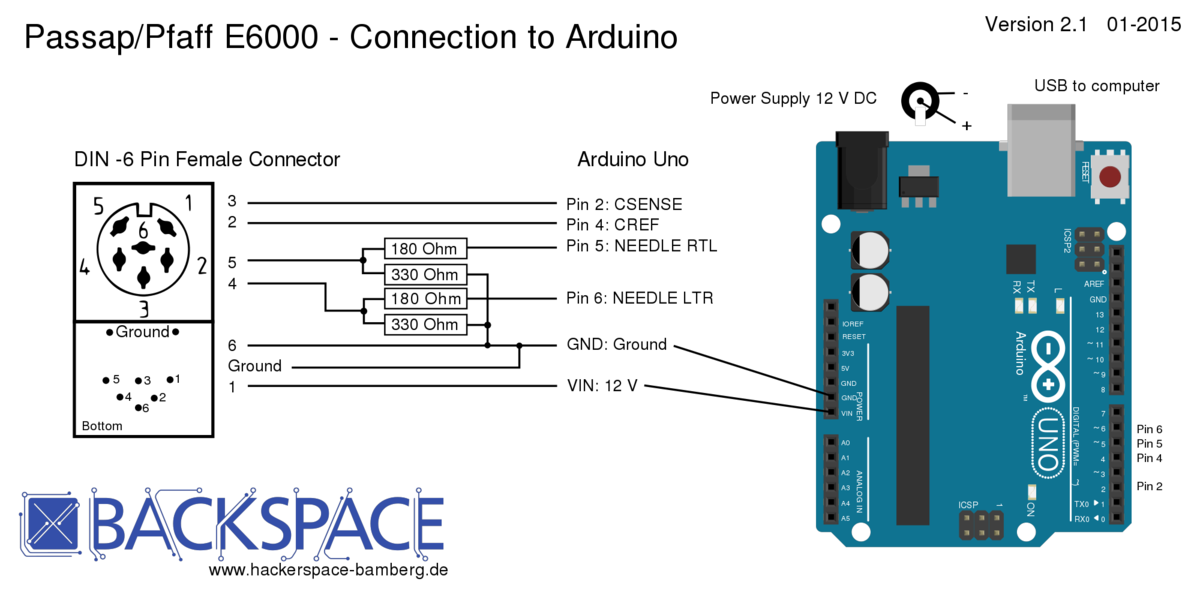
\includegraphics[width=0.75\linewidth]{myndir/bambergDIN6.png}
    \caption{Teikningar fyrir tengingu í gegnum DIN tengið (fengnar af vefsíðu Bamberg \cite{bamberg}). }
    \label{fig:bambergDIN6}
\end{figure}
Pinnar 2 og 4 taka við straum frá ljósaskynjurum sleðans. Pinnar 5 og 6 stýra stöðu seglana tveggja. 
Það er einn segull fyrir hvorra áttina. Sleðinn stillir munstur fyrir næstu umferð á meðan hann fer yfir nálarbeðið og prjónar  munstrið sem er nú þegar á nálarbeðinu. Til að snúa við seglunum þarf að minnsta kosti \textit{12v} straum. Pinnarnir senda merki um það hvort straumnum sé hleypt á seglanna eða ekki. \textit{Arduino} er öflug örtölva og hefur þann kost að hún er með hraða og skilvikra innri klukku. Örtölvan getur því einbeitt sér að því að taka við merkjum um stöðu ljósskynjaranna. 
Í hvert skipti sem staðan á ljósskynjaranum sem er tengdur í pinna númer 2 á \textit{Arduino} borðinu breytist þá er staðan á hinum skoðuð, sjá myndir \ref{fig:bambergDIN6}.% \& \ref{fig:PASSAPCONTROL}.

\begin{figure}[t]
    \centering
    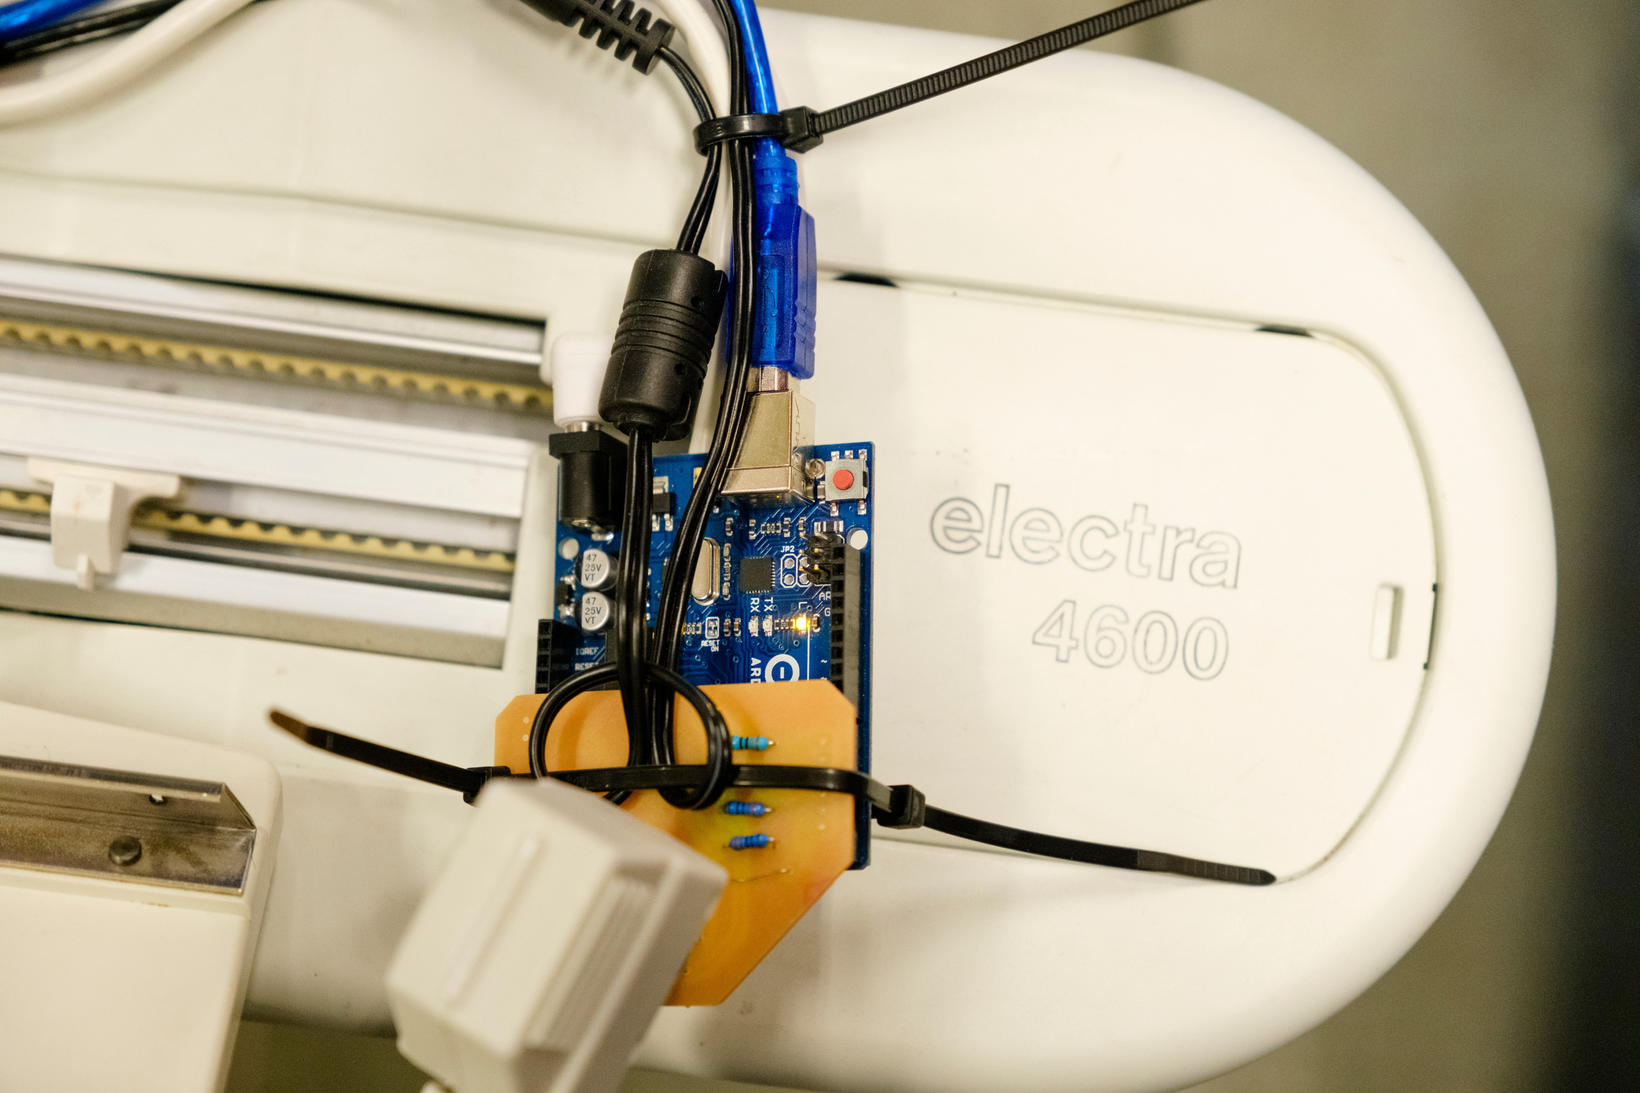
\includegraphics[width=0.7\linewidth]{myndir/elli/electra4600.jpg}
    \caption{\textit{Arduino} örtölva tengd við DIN-6 tengi á \textit{Passap E6000} - \textit{mbl.is/Kristinn Magnússon}}
    \label{fig:arduino}
\end{figure}
Það eru í raun tvö tilvik sem geta átt sér stað. Annaðhvort eru þeir í sömu stöðu eða í sitthvorri. Ef að aflestur ljósskynjara við breytingu á þeim sem er tendgur í pinna 2 er sú sama þá er við á leiðinni til hægri. Ef að þeir gefa sitthvort gildið þá erum við á leiðinni til vinstri. Örtölvan er því með innvortis teljara sem hækkar í gildi þegar aflesturinn er sá sami og lækkar þegar þeir gefa sitthvort gildið.

Nýja stýringin sem kemur í stað gamla stjórnborðsins hefur tvo meginliði örtölvuna og stýringin sem er keyrð á tölvu, sjá mynd \ref{fig:newConsole}. 

\begin{figure}[H]
    \centering
    \begin{tikzpicture}[auto, node distance=2cm, >=latex']
        \node [rectangle, draw, align=center] (arduino) {\textit{Arduino} örtölva};
        \node [rectangle, draw, align=center, right=4cm of arduino] (tlva) {tölva \\ keyrir stýringu};
        \node [rectangle, draw, align=center, below=4cm of arduino] (sled) {Sleði/Lás};
        \node [below=1cm of sled] (magnets) {};
        \node [left=1cm of sled] (light) {};
        \node [align=center, above=1cm of arduino] (power) {Spennubreytir};
        \node [rectangle, draw, align=center, above=1cm of tlva] (net) {Stjórnanda\\ vefviðmót};
        \node [align=center, below=1cm of tlva] (gagnagrunnur) {gagnagrunnur};
        \node [rectangle, draw, align=center, below=1cm of gagnagrunnur] (opid) {Opið\\ vefviðmót};
        \draw[-] (sled) edge[dotted, right] node[rotate=-90, above] {} (magnets)
                (sled) edge[dotted, right] node[rotate=-90, above] {} (light)
        
        
        ;
        \draw[->] 
(arduino) edge[dash dot, bend left] node[above] {\texttt{R} $\vee$ \texttt{L}} (tlva)
(tlva) edge[dash dot, bend left] node[below] {`\{byrjun\}\{munstur\}'} (arduino)
          (sled) edge[bend right] node[rotate=90, below] {lágur} (arduino)
          (sled) edge[bend right] node[rotate=90, above] {hár} (arduino)
                    (arduino) edge[->, bend right] node[align=center, rotate=90, below] {lágur} (sled)
          (arduino) edge[->, bend right] node[align=center, rotate=90, above] {hár} (sled)
          (power) edge[dashed,left] node[above] {} (arduino)
          (arduino) edge[dashed, left] node[left] {} (sled)
          (net) edge[<->,thick, dash dot dot] node[left] {} (tlva)
                    (gagnagrunnur) edge[<->,thick, dash dot dot] node[left] {} (tlva)
              (opid) edge[<->,thick, dash dot dot] node[left] {} (gagnagrunnur)

        ;

                \node[draw, rectangle, anchor=north west] at (2, -4) {
        \begin{tikzpicture}[x=1cm, y=0.8cm]
            \draw[thick] (0,0) -- (1,0) node[right] {5V};
             \draw[thick, dashed] (0,-0.5) -- (1,-0.5) node[right] {12V};
            \draw[thick, dash dot] (0,-1) -- (1,-1) node[right] {USB serial};
                        \draw[thick, dash dot dot] (0,-1.5) -- (1,-1.5) node[right] {Vefbeiðnir};
        \end{tikzpicture}};
    \end{tikzpicture}
    \caption{Kerfismynd af nýja stjórnborðið}
    \label{fig:newConsole}
\end{figure}

\begin{enumerate}
    \item \textbf{\textit{Arduino} örtölva} \begin{itemize}
        \item Sér um samskipti við sleðann með tengingu í gegnum DIN-6 tengi. Fær þaðan lestur af ljósskynjurum og stjórn á seglum. 
        \item Þegar skynjarinn sem er tengdur í pinna númer tvo breytir um gildi fer í gang truflun á kóðanum sem athugar um leið stöðuna á hinum ljósskynjaranum. Útfrá því fáum við út hvaða átt við erum að fara í. \begin{enumerate}
            \item Ef við fáum sitthvort gildið erum við að fara til vinstri. Teljari telur niður um einn.
            \item Ef við fáum sama gildið erum við að fara til hægri. Teljari telur upp um einn.
        \end{enumerate}
        \item Út frá innri teljaranum vitum við nákvæma staðsetningu sleðans á nálarbeðinu, svo lengi sem hann er tekinn útaf nálarbeðinu og setur aftur inná í hvert skipti sem örtölvan er endurræst/endurtengd.
        \item Örtölvan er skrifuð í C++ og hefur vigur með lengdina 179, eitt gildi fyrir hverja nál af nálarbeðinu. Það eru tvær aðrar breytur sem sjá um munstrin. Það er upphafs punktur og lengd munsturs. Grunngildin fyrir þau eru -10 og 10.
        \item Skilaboðin sem að \textit{Arduino} örtölvan sendir frá sér eru tvennskonar.
        \begin{enumerate}
            \item Ef að sleðin er vinstra megin við upphafs punktinn, teljari hefur gildi minna en upphafspunktsgildið. Þá er strengurinn \texttt{L} sendur yfir serial samskipti. 
            \item Ef að sleðin er hægra megin við punktinn sem er í fjarlægð lengd munstursins frá upphafspunktinnum, teljarinn hefur gildi sem er hææra en upphafspunktagildið lagt saman við lengd munstursins. Þá er strengurinn \texttt{R} sendur yfir serial samskipti.
        \end{enumerate}
        \item Þegar engin truflun á sér stað í keyrslu \textit{Arduino} örtölvunar þá ítrar hún fall sem athugar hvort einhver skilaboð hafi komið inn yfir serial tengi. Ef þau hafa komið inn, eru á strengjaformi sem hefur fleiri ein 3 stök þá er hann lesin sem staðlaður munsturs strengur. Þeir eru á forminu formerki serm er plús eða mínus. Síðan eru tveir tölustafir sem geta tekið gildi frá \texttt{01} upp í \texttt{90}. Þá loks kemur upp munstrið sem á að prjóna næstu umferð. Strengurinn hefur núll fyrir hverja nál sem á að prjóna lykkju.
        \begin{table}[H]
            \centering
	\begin{tabular}{|c|c|c|c|c|c|c|c|c|c|c|}
		\hline
		\multicolumn{1}{|c|}{\textbf{Formerki}} & \multicolumn{2}{c|}{\textbf{Upphafspunktur}} & \multicolumn{7}{c|}{\textbf{Munstur}} \\ 
		\hline
		- & 0 & 5 & 0 & 0 & 1 & 1 & 0 & 0 & 1 \\ 
		\hline
		\end{tabular}
            \caption{Sýnidæmi um löglegan munsturs sreng í serial samskiptum.}
            \label{tab:MunsturStrengur}
        \end{table}
        Formerkið gefur til kynna hvort megin við miðju nálarbeðsins munstrið á að byrja og upphafspunkturinn er númer nálar sem munstrið byrjar frá. Munstrið er alltaf skrifað frá vinstri til hægri.
    \end{itemize}
    \item \textbf{Tölvan sem keyrir stýringuna}
    Á vélinni þarf að vera uppset Node.js 20+, tenging með usb tengi við \textit{Arduino} örtölvuna.
    \begin{itemize}
        \item Stýringin sér um að geyma öll fylkin í heild sinni og matreiðir þá til \textit{Arduino} örtölvunar á réttu formi.
        \item Stýringin er alltaf að bíða eftir skilaboðum frá \textit{Arduino} örtölvunni. Þegar hún fær streng frá örtölvunni yfir serial samskipti athugar hún fyrst hvort það sé munstur að bíða eftir því að fara í vinnslu. Ef svo er þá er sía sem athugar ýmislegt en megin atriðið er hvort að næsta lína úr fylkinu sé oddatala eða ekki. \begin{enumerate}
            \item \texttt{L} sækir einungis næstu línu úr fylkinu ef númerlínunar er slétt. Sléttar tölur eru stilltar frá vinstri til hægri, hækkandi númer nála á nálarbeði. Þær eru síðan prjónar í öfuga átt.
            \item \texttt{R} sækir einungis næstu línu úr fylkinu ef númerlínunar er oddatala. Stilling og prjónun er í öfuga átt við \texttt{L}.
        \end{enumerate}
        \item Þegar munstur er senda á stýringuna er annað hvort:
        \begin{enumerate}
            \item Ekkert munstur í bið. Munstrið sett í minni og í vinnslu umleið.
            \item Munstur í vinnslu/bið og þá er nýja munstrinn bætt aftast í röðina.
        \end{enumerate}
        \item Stýringin hefur stjórnenda vefviðmót sem gefur notanda stýringar möguleika, eyða út munstrum, breyta upphafsnál o.s.frv. ásamt grafík sem sýnir núverandi stöðu vélarinar. Þar er hægt að sjá hvaða munstur er verið að stilla, hvað var stillt og hvað verður stillt næst.
        \item Stýringin tekur við munstrum í gegnum netbeiðnir, þær þurfa að innihalda upphafspunkt og munstursfylki. Munstursfylkin geta innihaldið tölugildi frá 0 til 4, eitt gildi fyrir hvern lit. Stýringin sér um að þýða fylkið og breytir öllum núllum í einn og öllum gildum í 0. Þá eru það gildin sem eru prjónuð.
        \item Bætt var við stýringar möguleika sem sækir munstur úr gagnagrunni ef ekkert munstur er í vinnslu eða bið.
        \item     \textbf{Opið vefviðmót}
    tekur við texta beiðnum frá notendum. Notfærir sér netsamskipti til að búa til mynd úr textanum með hjálp gervigreindar. Þá er bakgrunninn staðlaður. Myndin er síðan breytt í munstursfylki og vistað í gagnagrunni.       
    \end{itemize}
\end{enumerate}
\subsubsection{Stýring á mótor}
Passap vélarnar fóru í gegnum miklar framfarir á þeim tíma sem þær voru í framleiðslu. Upphaflega þurfti notandinn að stilla munstrinn sjálfur og færa sleðann. Snemma var komin lausn með mótor og einföldum breytingum á munstri með seglum. Mótorarnir breytust einnig og voru fyrstu stýrðir með fótapedölum. Síðan kom takkastýring sem bauð notendum á að stýra mótornum á þægilegri máta. Þetta hélt áfram lengi þar til \textit{Passap E6000} kom út með stjórnborðið sem gat gert allskyns munstur með hjálp innbyggðrar \textit{Form} tölvu. Hann hinsvegar tók yfir stjórn á tökkunum og þurfti í þeirri útfærslu að hafa stjórnborðið tengt og kveikt til að geta ýtt á takkanna. Þegar vélin var tekin í sundur kom í ljós að rafrásirnar af eldri útgáfunum eru enn til staðar og hægt er að tengja framhjá stjórnborðinu. Þá eru takkarnir aftur starfhæfir án stjórnborðsins. Kostir takkastýringarinar er að hún er skýr, einföld og notandi upplifir meiri stjórn á ferlinu.
\begin{figure}[H] % <- ekki taka út H þá fara myndirnar á flakk.
    \centering
    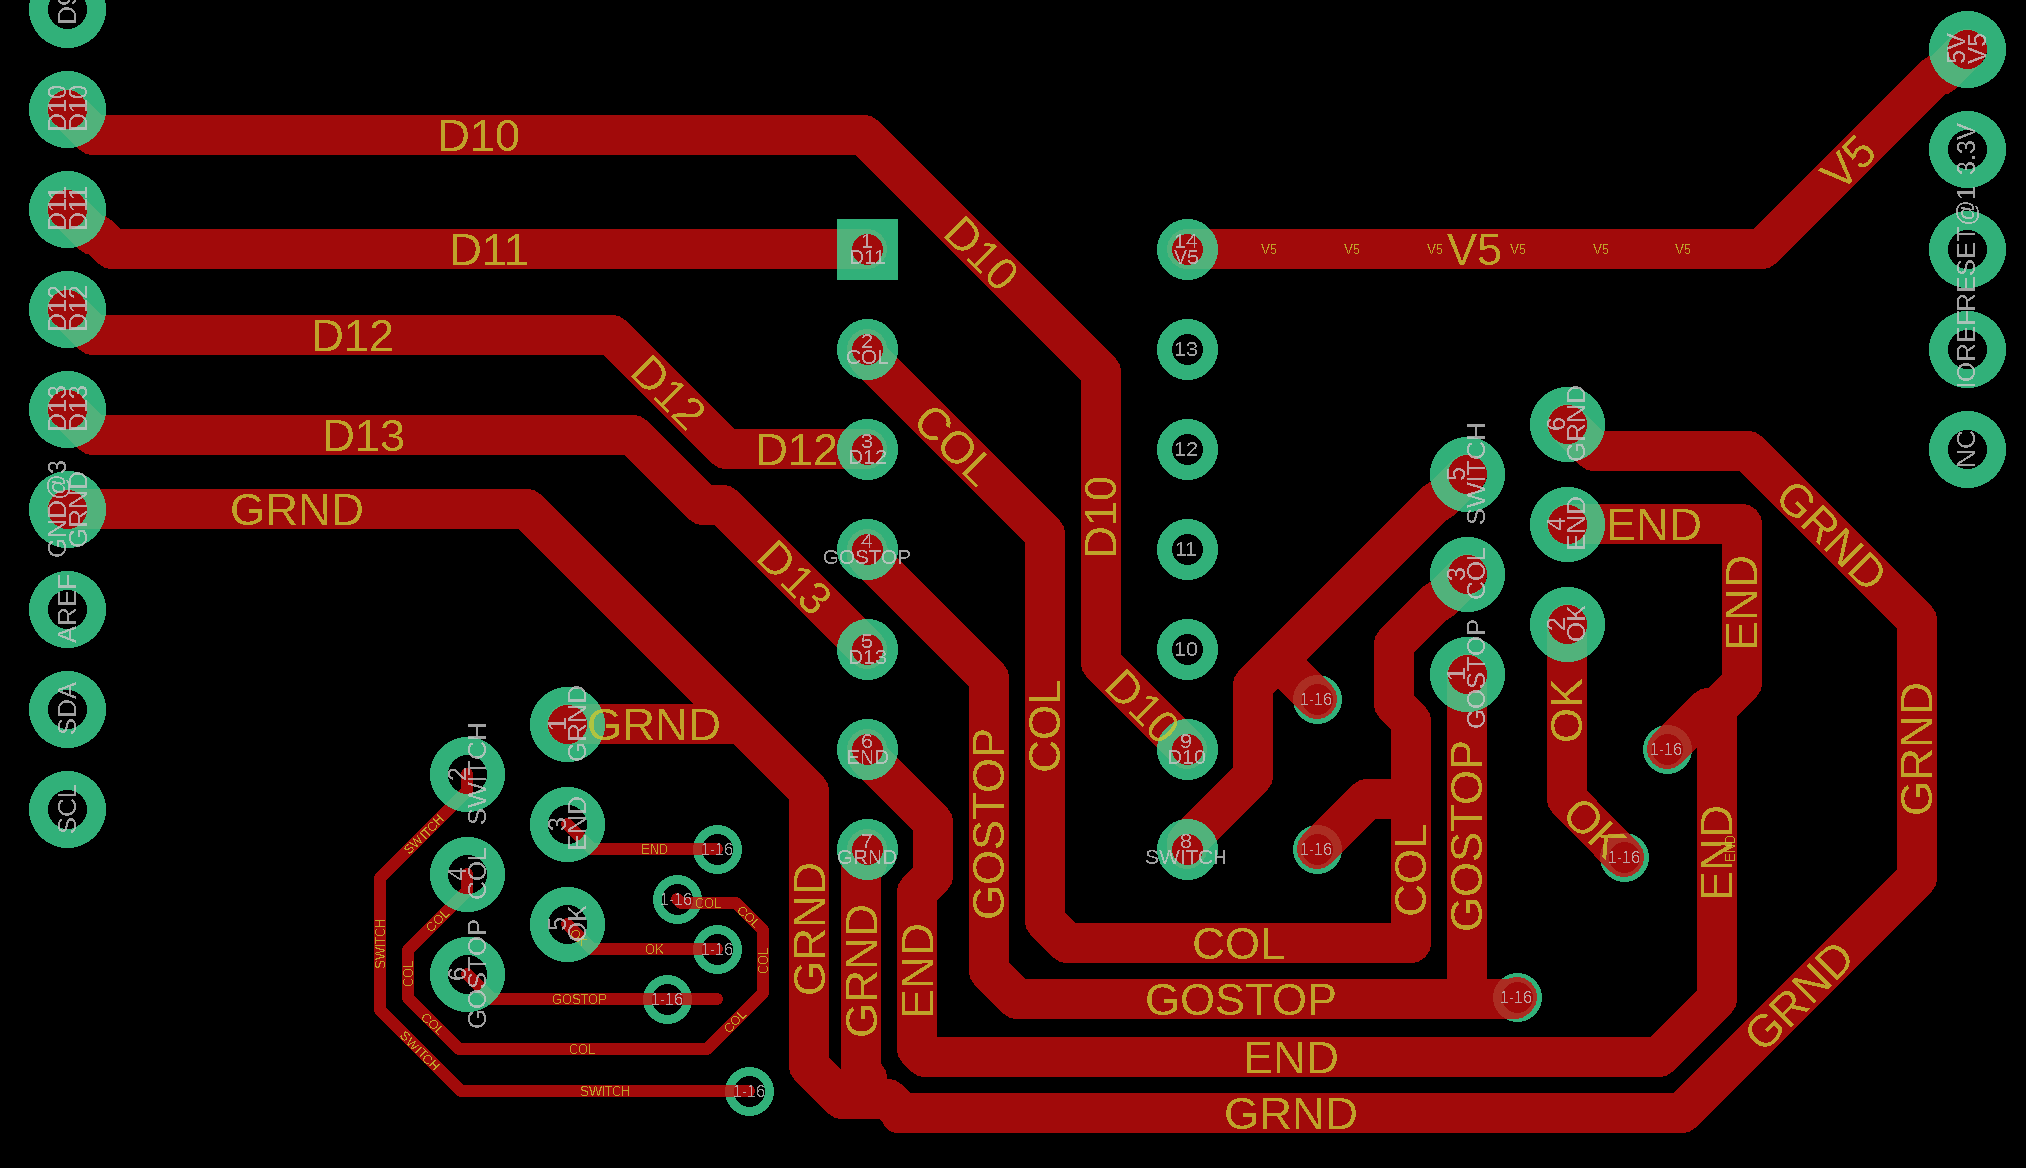
\includegraphics[width=0.75\linewidth]{myndir/PASSAPMOTOR.png}
    \caption{Rafrás sem tengir \textit{Arduino} við 7407N kubb sem tengist svo við 6pinna rj12 tengi til að stýra mótor. }
    \label{fig:PASSAPMOTOR}
\end{figure}
Til að stýra mótornum með \textit{Arduino} örtölvu er hægt að nota 7407N kubb í einfaldri rafrás sem tengir pinna frá örtölvunni við stýri pinna á 7407N og pinanna sem er stjórnað við rafrásir hvers takka. Takkarnir virka þannig að þeir eru alltaf með $5V$ straum á \textit{high} og þegar hann er tengdur í \textit{ground} er takkurinn virkur. 7407N hermir eftir því. Það er pláss fyrir skipanir í \textit{Arduino} kóðanum á strengjaformi sem hafa 3 stafi eða færri. 
Útfærsla á rafrás er hægt að sjá á mynd \ref{fig:PASSAPMOTOR}. Á myndinni af rafrásinni eru grænu jaðarpunktarnir til vinstri og hægri tenging við \textit{Arduino} örtölvuna sem sendir skilaboð á kubbinn. Kubburinn eru 14 samhverfu grænupunktarnir um miðjuna. Þeir taka við skipunum frá pinnum \textit{Arduino} örtölvunar á formi lágsstraums og þá er pinninn sem er fyrir neðan á myndinni tengdur í jörd (GRND). Þeir pinnar eru tengidr við rafrásir sem fara í 6 pinna rj12 tengi. Tengið sem er tengd út er til hægri við kubbinn. Þaðan eru send skilaboðin til mótorstýringarinnar. Vinstra megin við kubbinn er annað tengi sem er hægt að tengja við takkaborðið og þá helst virkni takkanna með viðbætri stýringu í gegnum \textit{Arduino} örtölvuna.
Í kóða er nú þegar skipunin \texttt{s} notuð til að slökkva og kveikja á mótor.
\subsubsection{Kóði}
Fyrir kerfið sem er á mynd \ref{fig:newConsole} voru gerð tvö repo sem eru í hýsingu hjá github. Þar er hægt að lesa og sækja allan kóðan sem er notaður til að stýra vélinni.
\begin{enumerate}
    \item \textbf{Stýringin}: \url{https://github.com/HiDefTextiles/passAPI}
    
        \begin{figure}[t] % <- ekki taka út H þá fara myndirnar á flakk.
    \centering
    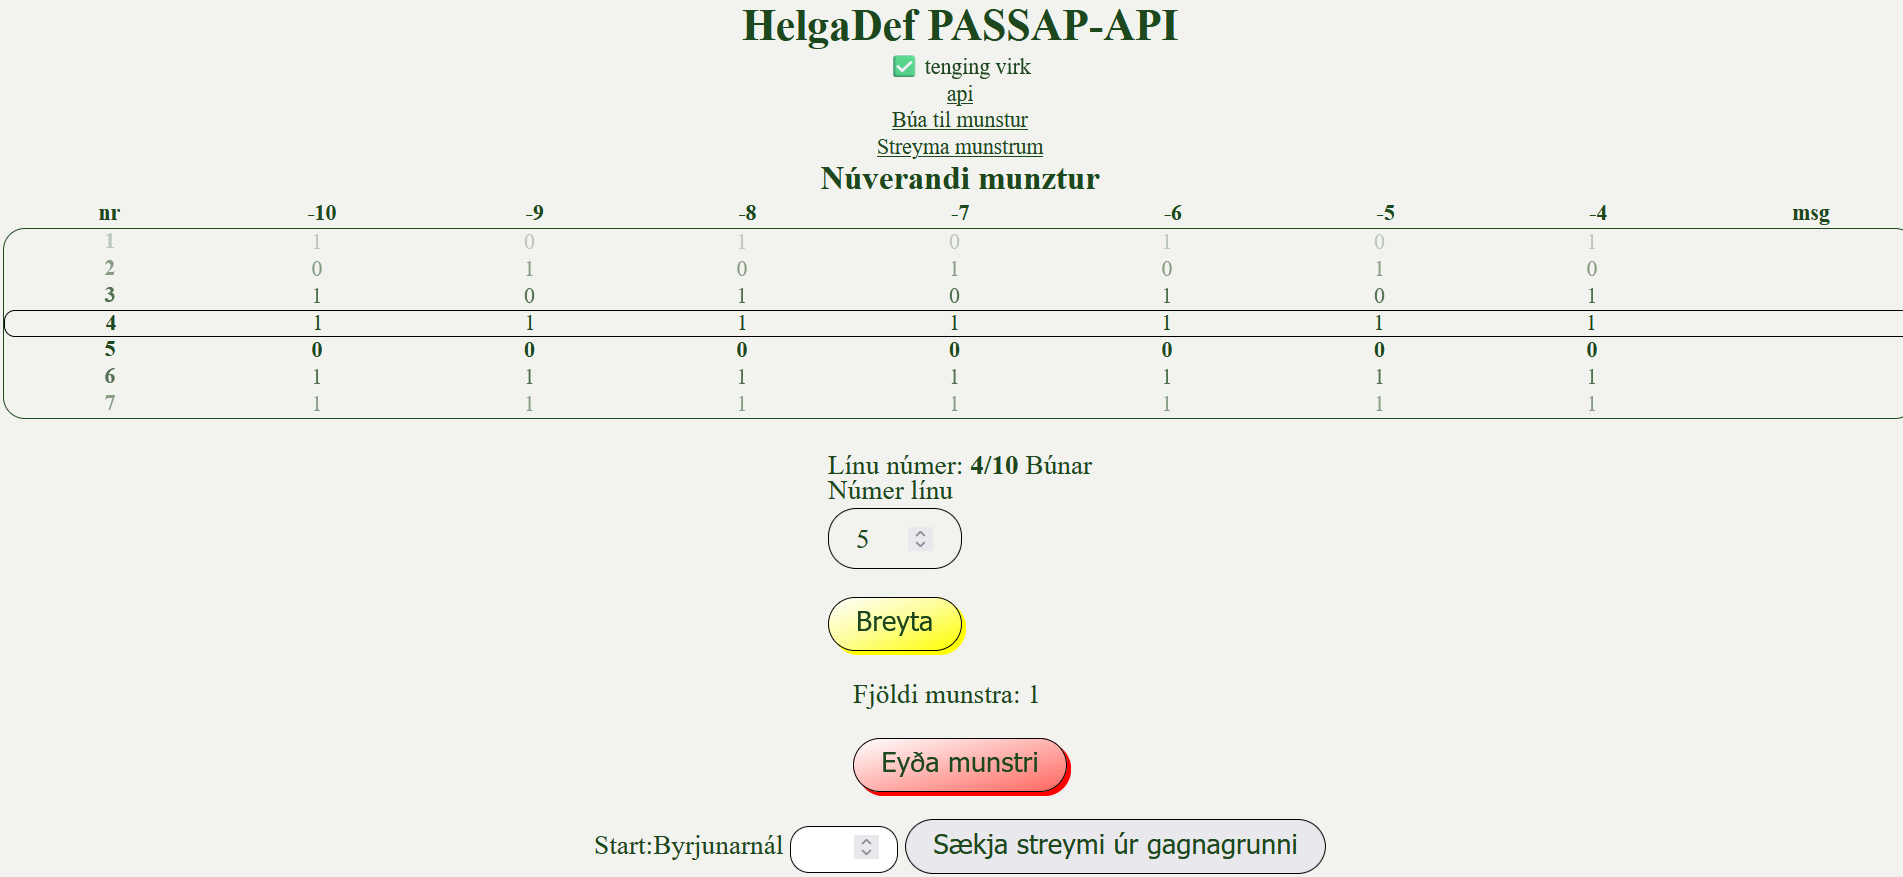
\includegraphics[width=0.8\linewidth]{myndir/passapiscreen.png}
    \caption{Stjórnanda vefviðmót stýringarinnar.}
    \label{fig:PASSAPMOTOR}
\end{figure}
    \begin{itemize}
        \item Þar er uppsett Node.js umhverfi í bæði typescript og javascript. Það þarf því að hafa Node.js 20+. Allir pakkarnir eru sóttir með skipuninni \texttt{npm install} og síðan er það keyrt með \texttt{npm run dev}. Ef það er ekki fundinn opin serial tenging við \textit{Arduino} þá ræsist ekki stýringin.
        \item     Inniheldur einnig kóðan fyrir \textit{Arduino} örtölvuna sem tekur við skipunum í gegnum serial samskipti og sendir út annaðhvort strenginn \texttt{R} eða \texttt{L} eftir tilvikum.
    \end{itemize}
    Inniheldur kóðan fyrir \textit{Arduino} örtölvuna sem tekur við skipunum í gegnum serial samskipti og sendir út annaðhvort strenginn \texttt{R} eða \texttt{L} eftir tilvikum.
    \item \textbf{Opið vefviðmót}: \url{https://github.com/tungufoss/passapnext} \\
    \begin{figure}[t] % <- ekki taka út H þá fara myndirnar á flakk.
    \centering
    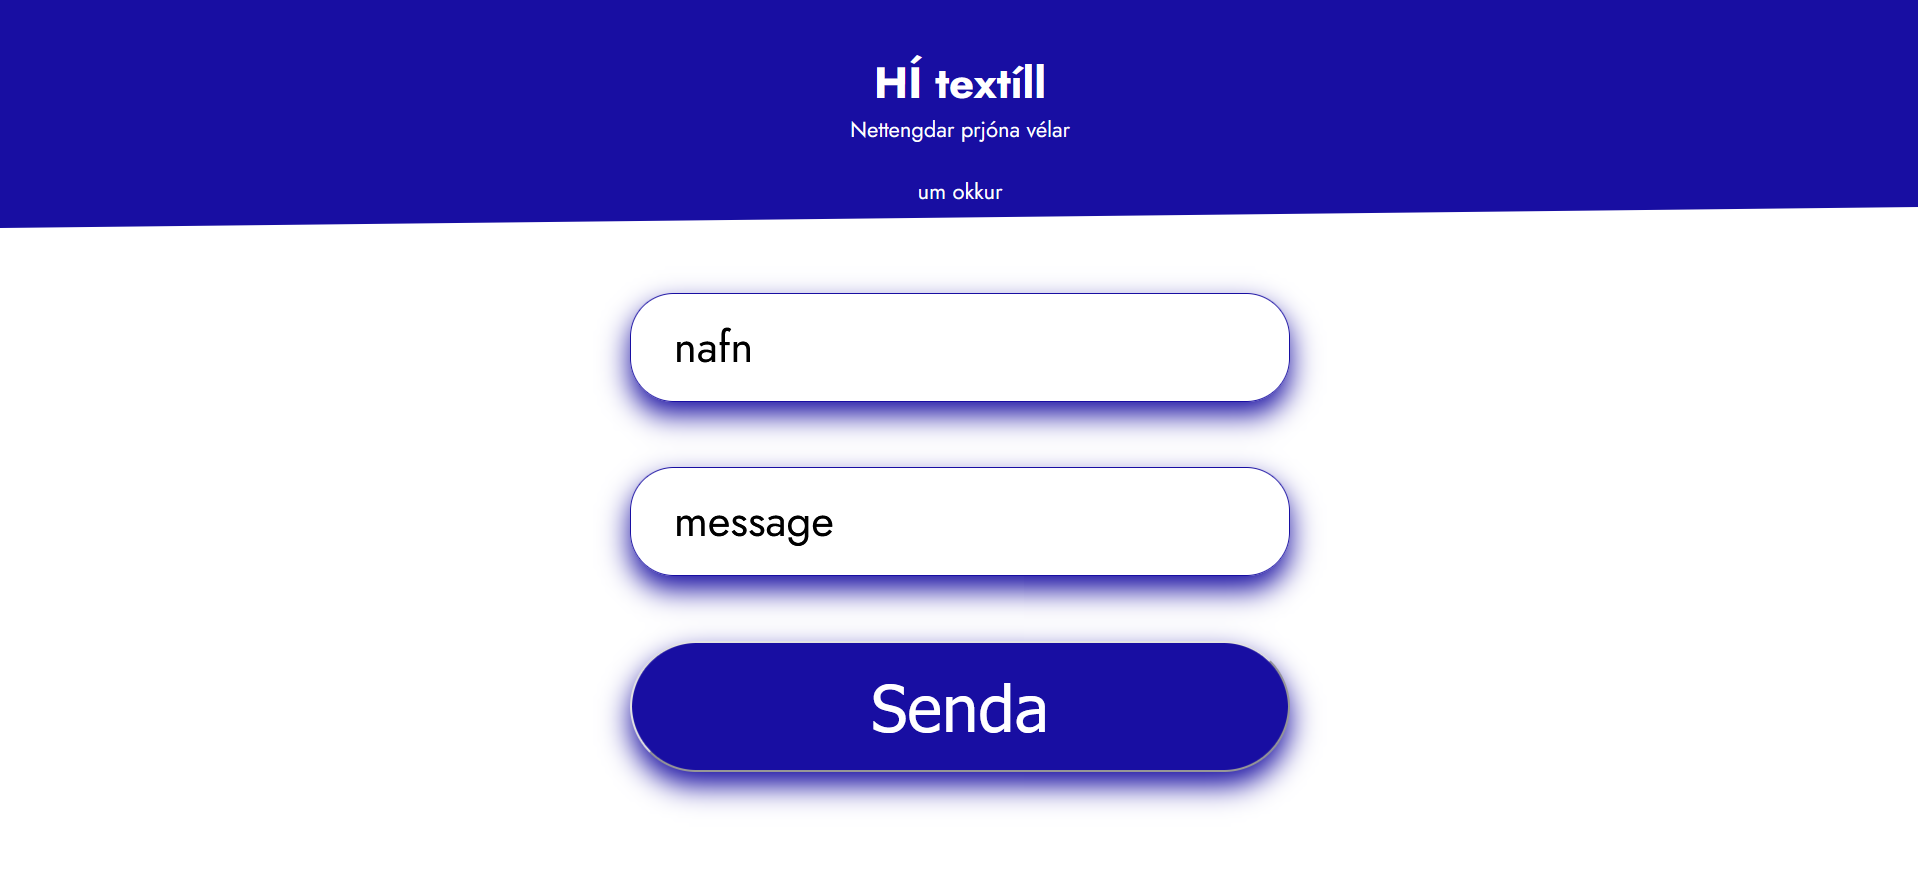
\includegraphics[width=0.8\linewidth]{myndir/passapnextscreen.png}
    \caption{Vefviðmótið sem tekur við beiðnum notenda fyrir hugmyndir að munstrum.}
    \label{fig:PASSAPMOTOR}
\end{figure}
    Þetta er uppsetning á vefsíðu með bakenda og framenda sem tekur við teksta og býr til mynda munstur útfrá teksta skilaboð sem eru vistuð í gagnagrunninn. Til að keyra það þarf að hafa eftirfarandi breytur í keyrslu umhverfinu.
    \begin{enumerate}
        \item \texttt{DATABASE\_URL=}\textit{Hlekkur fyrir samskipti við postgresSQL gagnagrunn}
        \item \texttt{YOUR\_ORG\_ID=} \textit{fengið frá openai API}.
        \item \texttt{PROJECT\_ID=} \textit{fengið frá openai API}.
        \item \texttt{OPENAI\_API\_KEY=} \textit{fengið frá openai API.}
    \end{enumerate}
\end{enumerate}
